\section{Аналіз існуючих підходів до вирішення задачі}
\subsection{Виділення об'єктів за допомоги віднімання фону}
Віднімання фону - процедура, що за умов нерухомості камери, оцінює зміну кожного пікселя зображення відносно фону, зображення якого було отримане раніше, та отримати в результаті бінарне зображення відмінності поточного зображення від зображення фону.

У вигляді математичних формул це виглядає так:

\begin{equation}
\label{eq:background_substraction}
P[F(t)] = P[I(t)] - P[B]
\end{equation}
де $P[B]$ - зображення фону, $P[I(t)]$ - поточне зображення, $P[F(t)]$ - різниця між поточним зображенням да фоном.

За умови незмінності фону можна працювати з формулою (\ref{eq:background_substraction}).

Для відслідковування рухів динамічних об'єктів також використовується рівняння:
\begin{equation}
\label{eq:frames_difference}
\|P[F(t)] - P[F(t+1)]\| > Treshold
\end{equation}
де $Treshold$ - деяка задана порогова величина.

\begin{figure}[H]
	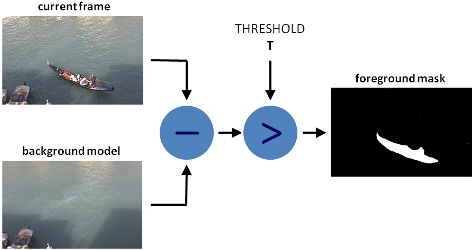
\includegraphics[width=0.9\linewidth]{task_analysis/img/background_substraction}
	\caption{Ілюстрація роботи простого алгоритма віднімання фону}
\end{figure}

Алгоритм дійсний як для кольорових зображень, так і для зображень у відтінках сірого.

Переваги цього алгоритму у тому, що його достатньо просто реалізувати та він не потребує складних обчислень ( більшість операцій можна векторизувати та паралелізувати що значно прискорює швидкість обробки ). Проте його найбільшим недоліком можна вважати те, що за його допомоги неможливо виділити об'єкт на динамічному фоні, він зпродукує велику кількість областей для подальшого аналізу, який може бути вже не таким тривіальним і система на його базі не зможе працювати в режимі on-line.

\subsection{Відслідковування руки за допомоги контролерів}

У минулих століттях саме цей підхід для роботи з відслідковуванням руки та аналізу жестів був популярним через достатньо прозору та просту програмну реалізацію. За допомоги приблизно 16 сенсорів та вбудованого в рукавицю гіроскопа можна достатньо точно відслідковувати навіть мікрорухи руки.

\begin{figure}[H]
	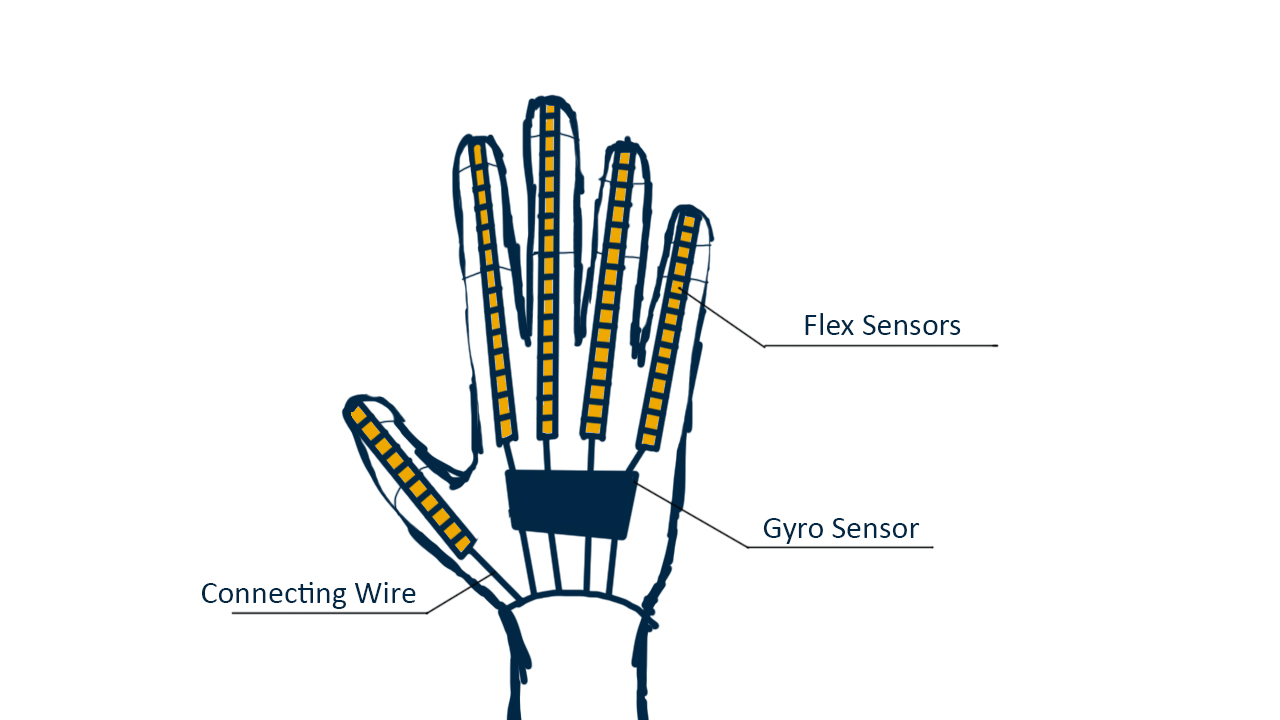
\includegraphics[width=0.9\linewidth]{task_analysis/img/wired_glove}
	\caption{Cхема рукавиці з сенсорами}
\end{figure}

З точки зору розробників ПЗ простота була у тому, що на вхід вони вже мали позиції усіх ключових точок руки відносно центру ( найчастіше це була лодоня ), та положення центру у просторі. Для аналізу статичних жестів достатньо мати лише відносне положення усіх ключових точок відносно центру. Для аналізу динамічних жестів вже потрібні дані зміни положення руки у просторі.

Також були прототипи контролерів, що містили лише гіроскоп, проте відслідковування позиції у просторі руки як одного об'єкта без данних про позиції ключових точок на пальцях виявився нікому непотрібним і контролели швидко вийшли з виробництва.

Переваги цього підходу до відслідковування руки у просторі в тому, що він дає дуже точні результати та з мінімальною затримкою, проте він має дуже серйозний недоліки - потреба в носінні на собі додаткових незручних приладів та складність підтримки і ремонту таких девайсів.

\subsection{Колірні фільтри для детекції шкіри на зображенні}

Оскільки будь-яке цифрове зображення можливо представити у вигляді:

\begin{equation}
	\label{eq:digital_image_representation}
	M = matrix \: W \times H \times D \: , \: d = dimD
\end{equation}

де $M$ - цифрове зображення, $W$ - ширина зображення, $D$ - розмір колірного простору.
Наприклад для типових колірних просторів RGB, HSV, YCrCb $d = 3$. Для колірного простору градацій сірого $d = 1$.

Колірний простір можна представити так:
\begin{equation}
	\label{eq:color_space_representation}
	( x=(x_1,...,x_d) \in D) \Leftrightarrow ( 0<=x_1<=d_1, ... , 0<=x_d<=d_d )	
\end{equation}
де $D$ - колірний простір, $d_1,...,d_d$ - обмеження координат колірного простору.

Найчастіше зустрічається випадок коли $x_i \in \mathbb{N} \cup \{0\}, d_i = 2^8 , i=1..d$ оскільки це списується в принцип збереження данних у пам'яті ПК.


\subsubsection{Прості колірні фільтри}
Основний принцип роботи простих колірних фільтрів полягає у тому, що емпірічними методами виділяється гіперкуб, що повністю містить у собі всі можливі значення пікселей, що характеризували певний об'єкт.

Формальний вигляд простого фільтра:
\begin{equation}
	\label{eq:simple_color_filter}
	H = {x \in D \mid a_i <= x_i <= b_i, i=1..d}
\end{equation}
	де $a_i,b_i$ - грані гіперкуба.
	
Прості колірні фільтри хороші тим, що дуже прості в реалізації, швидко працюють та є можливість паралелізації обчислень оскільки фільтр обробряє кожен піксель незалежно.

Результатом роботи колірного фільтра $H$ зображення $M$ є бінарна матриця $Q$ :
\begin{equation}
	\label{eq:simple_color_filter_result}
	Q = [q_{ij}], \:\: q_{ij} = ( M[i,j] \in H ), i=1..dimW, j=1..dimH
\end{equation}
Тобто матриця $q_{ij} \in \{0,1\} \forall i,j$ і тому можна достатньо просто записати композицію простих фільтьтрів як поелементні бінарні операції над матрицями. Звісно за допомоги кубів можливо апроксимувати достатньо точно найскладніші фігури, проте це має свої слабкі сторони:
\begin{enumerate}
	\item апроксимація певного тіла кубами в просторі розмірності $d$ достатньо нетривіальна задача з точки зору математики
	\item зі збільшенням точності буде рости кількість простих колірних фільтрів у ланцюгу композицій і це призведе до падіння швидкості роботи
\end{enumerate}

\subsubsection{Гаусівська модель}

Одним з більш складних підходів є припущення, що ймовірність належності кольору пікселя до множини кольорів певного об'єкта є деяка випадкова величина, що розподілена за гаусівським законом розподілу \cite{AdaptiveBigaussian}.

Також цей підхід враховує змінні умови освітлення шляхом поеднання двух гаусівських моделей. Перша гаусівська модель будується у спеціальних умовах звичайного освітлення, друга - при черезмірному освітленні.

Алгоритм навчання такої моделі - метод вибору математичного сподівання та кореляційної матриці.

Класифікація проводиться згідно з вибраною довірчою ймовірністю. У конкретному випадку колірного простору розміності 2 це буде еліпс.

Основним недоліком цього підходу є те, що на практиці достатньо важко правильно підібрати математичне сподівання та кореляційну матрицю і тому точність методу недостатня.

\subsubsection{Байесовська модель}

Цей підхід зустрічається у літературі не дуже часто і основна формула, що описує модель, на перший погляд незрозуміла:
\begin{equation}
\label{eq:bayesian_classifier}
P(s|c) = \frac{P(c|s) * P(s)}{P(c)}
\end{equation}

Це звичайний запис теореми Байеса для знаходження апостеріорних ймовірностей.

$P(s|c)$ - ймовірність того, що піксель належить до множини кольорів шуканого об'єкта за умови що піксель має колір $c$. $P(s|c)$ в свою чергу має обернене формулювання - ймовірність того, що піксель приймає значення $c$ за умови що він належить до множини кольорів об'єкта.
$P(s)$ - ймовірність того, що піксель належить до множини кольорів об'єкта. $P(c)$ - загальна ймовірність того, що піксель має колір $c$.

Прочитавши такі формулювання складно взагалі зрозуміти як обрахувати ймовірності що стоять по праву сторону від рівності.

Основне припущення цього підходу - кольори окремих пікселей на рображенні незалежні один від одного. За такого припущення можна сказати, що $P(s)/P(c)$ - деяка загальна константа якою можна знехтувати поставивши її рівною 1, а $P(c|s) = m/n$, де $m$ - кількість пікселів кольору $c$, що належать об'єкту, $n$ - загальна кількість пікселів, що належала об'єкту.

Навчання такої моделі можна розбити на 2 етапи:
\begin{enumerate}
	\item Обробка зображення для навчання - на зображеннях призначених для навчання замальовуються усі сторонні елементи окрім шкіри і таким чином формується маска зображення.
	\item Навчання - підраховується кількість кожного пікселя що потрапляє у область шкіри на зображенні та в кінці навчання ділиться на загальну кількість пікселів, що належали шкірі.
\end{enumerate}

Таким чином побудована функція, що ставить у відповідність елементам колірного простору величину на проміжку $[0,1]$. У випадках розмірностей 1 чи 2 можливо побудувати графік цієї функції для аналізу навчання моделі.